\documentclass{article}
\usepackage{tikz}
\usepackage{xcolor}
\usepackage{amssymb}
\usetikzlibrary{patterns, positioning, arrows.meta, shapes.geometric, calc, backgrounds, decorations.pathreplacing}

% ============= MODERN COLOR PALETTE =============
% Indigo tones for prompts
\definecolor{promptFill}{HTML}{818CF8}
\definecolor{promptBorder}{HTML}{4F46E5}

% Slate tones for masks
\definecolor{maskFill}{HTML}{CBD5E1}
\definecolor{maskBorder}{HTML}{64748B}
\definecolor{maskPattern}{HTML}{475569}

% Amber/Orange tones for predicted tokens  
\definecolor{predictedFill}{HTML}{FCD34D}
\definecolor{predictedBorder}{HTML}{F59E0B}
\definecolor{predictedPattern}{HTML}{D97706}

% Emerald tones for denoised/final tokens
\definecolor{denoisedFill}{HTML}{6EE7B7}
\definecolor{denoisedBorder}{HTML}{10B981}

% Rose tones for removed tokens
\definecolor{removedFill}{HTML}{FECDD3}
\definecolor{removedBorder}{HTML}{F43F5E}
\definecolor{removedPattern}{HTML}{E11D48}

% UI colors
\definecolor{blueBox}{HTML}{3B82F6}
\definecolor{blueBg}{HTML}{EFF6FF}
\definecolor{greenBox}{HTML}{10B981}
\definecolor{greenBg}{HTML}{ECFDF5}
\definecolor{cropRed}{HTML}{DC2626}
\definecolor{textDark}{HTML}{1E293B}
\definecolor{textMuted}{HTML}{64748B}

\begin{document}

\begin{figure*}[t]
\centering
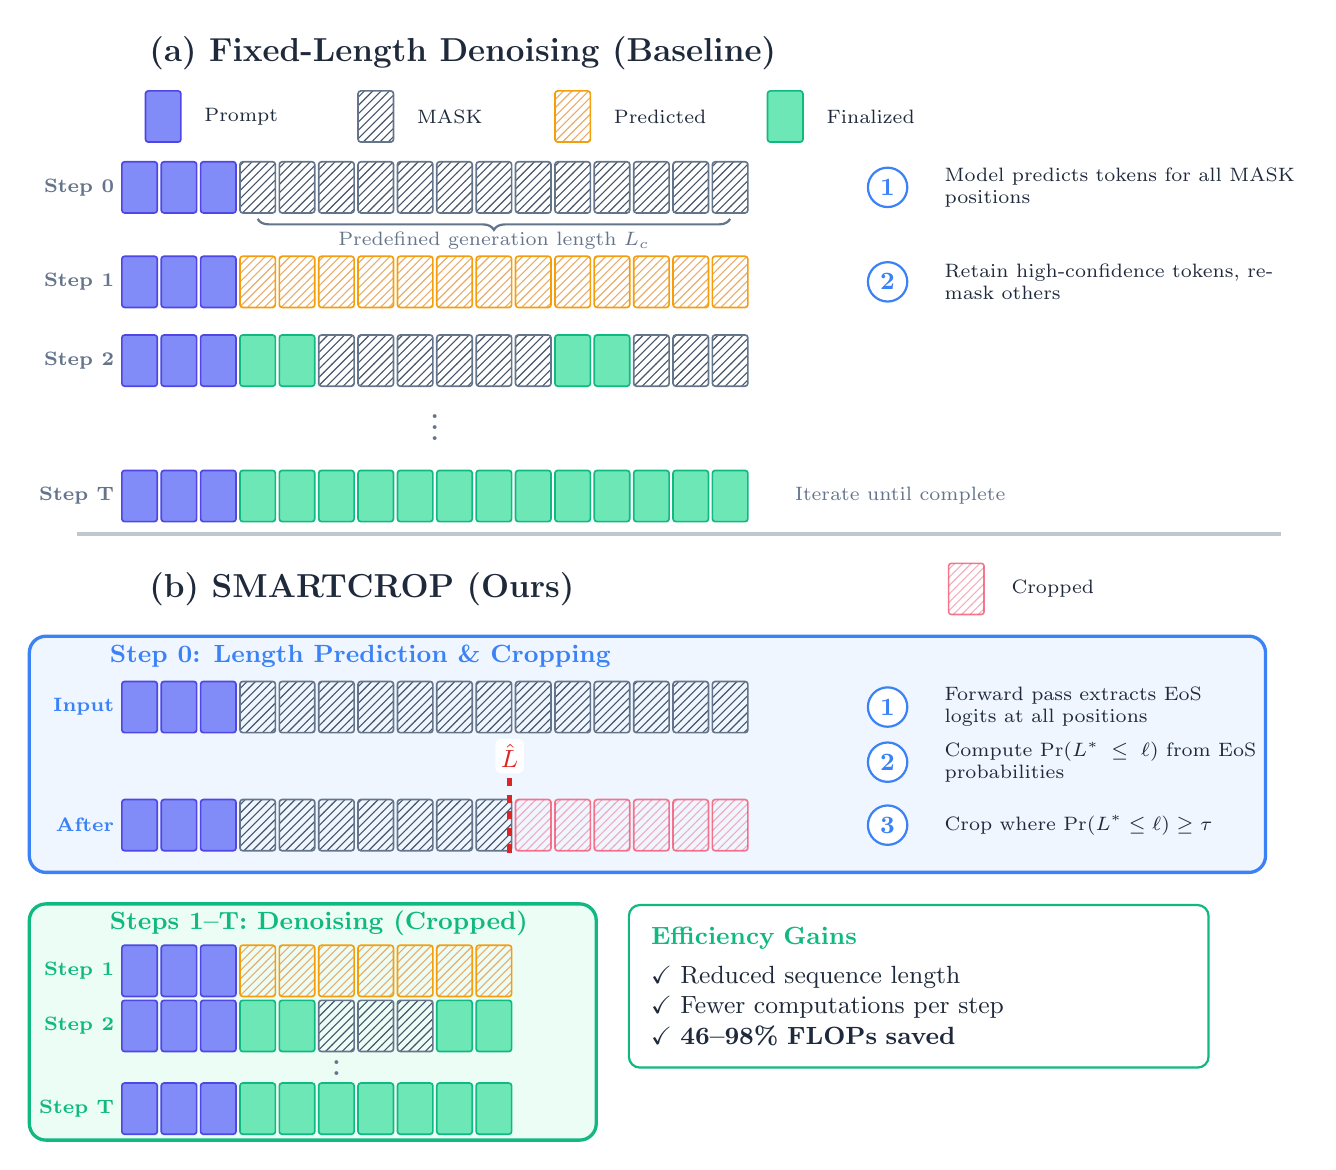
\begin{tikzpicture}[
    % Base token style with shadow
    token/.style={
        draw, 
        minimum width=0.45cm, 
        minimum height=0.65cm, 
        outer sep=0,
        rounded corners=1pt,
        line width=0.6pt
    },
    % Prompt tokens - indigo
    prompt/.style={
        token, 
        fill=promptFill, 
        draw=promptBorder
    },
    % Mask tokens - slate with pattern
    mask/.style={
        token, 
        fill=maskFill, 
        draw=maskBorder,
        pattern=north east lines, 
        pattern color=maskPattern
    },
    % Predicted tokens - amber with subtle pattern
    predicted/.style={
        token, 
        fill=predictedFill, 
        draw=predictedBorder,
        pattern=north east lines, 
        pattern color=predictedPattern!60
    },
    % Denoised tokens - emerald
    denoised/.style={
        token, 
        fill=denoisedFill, 
        draw=denoisedBorder
    },
    % Removed tokens - rose with pattern
    removed/.style={
        token, 
        fill=removedFill, 
        draw=removedBorder,
        pattern=north east lines, 
        pattern color=removedPattern!50,
        opacity=0.7
    },
    % Arrow style
    arrow/.style={
        -{Stealth[length=2.5mm, width=2mm]}, 
        line width=1pt, 
        cropRed
    },
    % Annotation circles
    annotation/.style={
        circle, 
        draw=blueBox, 
        fill=white, 
        line width=0.8pt,
        inner sep=1.5pt, 
        minimum size=0.5cm, 
        font=\small\bfseries,
        text=blueBox
    },
    % Section headers
    sectiontitle/.style={
        font=\large\bfseries,
        text=textDark
    },
    % Step labels
    steplabel/.style={
        font=\scriptsize\bfseries,
        text=textMuted
    },
    % Description text
    desctext/.style={
        font=\scriptsize,
        text=textDark
    }
]

% ============= PANEL (a): BASELINE =============
\node[sectiontitle, anchor=west] at (0, 5.8) {(a) Fixed-Length Denoising (Baseline)};

% Legend for panel (a) - with better spacing and labels
\node[prompt] at (0.3, 5.0) {};
\node[desctext, anchor=west] at (0.7, 5.0) {Prompt};

\node[mask] at (3.0, 5.0) {};
\node[desctext, anchor=west] at (3.4, 5.0) {MASK};

\node[predicted] at (5.5, 5.0) {};
\node[desctext, anchor=west] at (5.9, 5.0) {Predicted};

\node[denoised] at (8.2, 5.0) {};
\node[desctext, anchor=west] at (8.6, 5.0) {Finalized};

% Row 1: Initial state
\node[steplabel, anchor=east] at (-0.2, 4.1) {Step 0};
\foreach \i in {0,1,2} { \node[prompt] at (\i*0.5, 4.1) {}; }
\foreach \i in {3,...,15} { \node[mask] at (\i*0.5, 4.1) {}; }

% Brace for predefined length
\draw[decorate, decoration={brace, amplitude=4pt, mirror}, line width=0.8pt, textMuted] 
    (1.5, 3.7) -- (7.5, 3.7) node[midway, below=1pt, font=\scriptsize, text=textMuted] {Predefined generation length $L_c$};

% Annotation 1
\node[annotation] at (9.5, 4.1) {1};
\node[desctext, anchor=west, text width=4.5cm] at (10.1, 4.1) {Model predicts tokens for all MASK positions};

% Row 2: First prediction
\node[steplabel, anchor=east] at (-0.2, 2.9) {Step 1};
\foreach \i in {0,1,2} { \node[prompt] at (\i*0.5, 2.9) {}; }
\foreach \i in {3,...,15} { \node[predicted] at (\i*0.5, 2.9) {}; }

% Annotation 2
\node[annotation] at (9.5, 2.9) {2};
\node[desctext, anchor=west, text width=4.5cm] at (10.1, 2.9) {Retain high-confidence tokens, remask others};

% Row 3: Partial denoising
\node[steplabel, anchor=east] at (-0.2, 1.9) {Step 2};
\foreach \i in {0,1,2} { \node[prompt] at (\i*0.5, 1.9) {}; }
\foreach \i in {3,4} { \node[denoised] at (\i*0.5, 1.9) {}; }
\foreach \i in {5,...,10} { \node[mask] at (\i*0.5, 1.9) {}; }
\foreach \i in {11,12} { \node[denoised] at (\i*0.5, 1.9) {}; }
\foreach \i in {13,...,15} { \node[mask] at (\i*0.5, 1.9) {}; }

% Dots
\node[text=textMuted] at (3.75, 1.15) {\Large$\vdots$};

% Row 4: Final result
\node[steplabel, anchor=east] at (-0.2, 0.18) {Step T};
\foreach \i in {0,1,2} { \node[prompt] at (\i*0.5, 0.18) {}; }
\foreach \i in {3,...,15} { \node[denoised] at (\i*0.5, 0.18) {}; }
\node[desctext, anchor=west, text=textMuted] at (8.2, 0.18) {Iterate until complete};

% ============= SEPARATOR =============
\draw[line width=1.5pt, textMuted!40] (-0.8, -0.3) -- (14.5, -0.3);

% ============= PANEL (b): SMARTCROP =============
\node[sectiontitle, anchor=west] at (0, -1.0) {(b) SMARTCROP (Ours)};

% Additional legend item for removed
\node[removed] at (10.5, -1.0) {};
\node[desctext, anchor=west] at (10.95, -1.0) {Cropped};

% Stage 1: Initial Length Adjustment - Blue box
\begin{scope}[on background layer]
    \fill[blueBg, rounded corners=6pt] (-1.4, -1.6) rectangle (14.3, -4.6);
\end{scope}
\draw[blueBox, line width=1.2pt, rounded corners=6pt] (-1.4, -1.6) rectangle (14.3, -4.6);
\node[font=\small\bfseries, text=blueBox, anchor=west] at (-0.5, -1.85) {Step 0: Length Prediction \& Cropping};

% Row 1: Initial forward pass
\node[steplabel, anchor=east, text=blueBox] at (-0.2, -2.5) {Input};
\foreach \i in {0,1,2} { \node[prompt] at (\i*0.5, -2.5) {}; }
\foreach \i in {3,...,15} { \node[mask] at (\i*0.5, -2.5) {}; }

% Annotations for step 0
\node[annotation] at (9.5, -2.5) {1};
\node[desctext, anchor=west, text width=3.8cm] at (10.1, -2.5) {Forward pass extracts EoS logits at all positions};

\node[annotation] at (9.5, -3.2) {2};
\node[desctext, anchor=west, text width=4.5cm] at (10.1, -3.2) {Compute $\Pr(L^* \leq \ell)$ from EoS probabilities};

% Row 2: After cropping
\node[steplabel, anchor=east, text=blueBox] at (-0.2, -4.0) {After};
\foreach \i in {0,1,2} { \node[prompt] at (\i*0.5, -4.0) {}; }
\foreach \i in {3,...,9} { \node[mask] at (\i*0.5, -4.0) {}; }
\foreach \i in {10,...,15} { \node[removed] at (\i*0.5, -4.0) {}; }

% Crop indicator - more prominent
\draw[cropRed, line width=2pt, dashed] (4.7, -3.4) -- (4.7, -4.45);
\node[font=\small\bfseries, text=cropRed, anchor=south, fill=white, inner sep=2pt, rounded corners=2pt] at (4.7, -3.35) {$\hat{L}$};

\node[annotation] at (9.5, -4.0) {3};
\node[desctext, anchor=west, text width=4.5cm] at (10.1, -4.0) {Crop where $\Pr(L^* \leq \ell) \geq \tau$};

% Stage 2: Standard Denoising - Green box
\begin{scope}[on background layer]
    \fill[greenBg, rounded corners=6pt] (-1.4, -5.0) rectangle (5.8, -8.0);
\end{scope}
\draw[greenBox, line width=1.2pt, rounded corners=6pt] (-1.4, -5.0) rectangle (5.8, -8.0);
\node[font=\small\bfseries, text=greenBox, anchor=west] at (-0.5, -5.25) {Steps 1–T: Denoising (Cropped)};

% Row 3: Denoising step 1
\node[steplabel, anchor=east, text=greenBox] at (-0.2, -5.85) {Step 1};
\foreach \i in {0,1,2} { \node[prompt] at (\i*0.5, -5.85) {}; }
\foreach \i in {3,...,9} { \node[predicted] at (\i*0.5, -5.85) {}; }

% Row 4: Denoising step 2
\node[steplabel, anchor=east, text=greenBox] at (-0.2, -6.55) {Step 2};
\foreach \i in {0,1,2} { \node[prompt] at (\i*0.5, -6.55) {}; }
\foreach \i in {3,4} { \node[denoised] at (\i*0.5, -6.55) {}; }
\foreach \i in {5,6,7} { \node[mask] at (\i*0.5, -6.55) {}; }
\foreach \i in {8,9} { \node[denoised] at (\i*0.5, -6.55) {}; }

% Dots
\node[text=textMuted] at (2.5, -7.05) {\Large$\vdots$};

% Row 5: Final
\node[steplabel, anchor=east, text=greenBox] at (-0.2, -7.6) {Step T};
\foreach \i in {0,1,2} { \node[prompt] at (\i*0.5, -7.6) {}; }
\foreach \i in {3,...,9} { \node[denoised] at (\i*0.5, -7.6) {}; }

% Efficiency annotation - styled box
\node[
    draw=greenBox, 
    fill=white, 
    rounded corners=4pt, 
    line width=0.8pt,
    font=\small, 
    anchor=north west, 
    text width=6.8cm, 
    align=left,
    inner sep=8pt
] at (6.2, -5.0) {
    \textbf{\textcolor{greenBox}{Efficiency Gains}}\\[3pt]
    \textcolor{textDark}{{\small$\checkmark$} Reduced sequence length}\\
    \textcolor{textDark}{{\small$\checkmark$} Fewer computations per step}\\
    \textcolor{textDark}{{\small$\checkmark$} \textbf{46–98\% FLOPs saved}}
};

\end{tikzpicture}
\caption{\textbf{Comparison of diffusion decoding strategies.} 
\textbf{(a) Fixed-Length Denoising (Baseline):} Standard masked diffusion processes the full context window $L_c$ for all denoising steps. 
\textbf{(b) SMARTCROP:} Our method performs an initial forward pass to extract EoS logits, computes cumulative probability Pr($L^* \leq \ell$), identifies predicted length $\hat{L}$ at threshold $\tau$, and crops the context before denoising begins. This one-shot adjustment eliminates computational waste while maintaining output quality.}
\label{fig:method}
\end{figure*}

\end{document}